\chapter{The 1PI Renormalization Group}
\label{ch:volume-ii-1pi-renormalization-group}

\section{Scale-Dependent Coordinates on the 1PI Effective Action}

The previous chapters constructed local counterterms and organized
subdivergence subtractions.  We now use that construction to compare
renormalized 1PI data at different Euclidean momentum scales.

Work in a Euclidean perturbative quantum field theory on \(\R^D\), with a UV
regulator denoted by \(\Lambda\).  Let \(\Gamma_\Lambda[\varphi]\) be the
regulated 1PI effective action, expressed as a functional of a classical field
\(\varphi\).  Its momentum-space expansion has the form
\[
  \Gamma_\Lambda[\varphi]
  =
  \sum_{n\ge0}\frac1{n!}
  \int
  \prod_{a=1}^n\frac{\dd^D k_a}{(2\pi)^D}\,
  (2\pi)^D\delta\!\left(\sum_{a=1}^n k_a\right)
  \Gamma_\Lambda^{(n)}(k_1,\ldots,k_n)
  \widehat\varphi(k_1)\cdots\widehat\varphi(k_n).
\]
The distribution \(\Gamma_\Lambda^{(n)}\) is the regulated 1PI \(n\)-point
vertex.  Momentum conservation allows one momentum argument to be suppressed
when convenient.

A scale-dependent 1PI coordinate is obtained by specifying:
\begin{itemize}
  \item a finite list of local operators \(\mathcal O_I\), each with a number
  \(n_I\) of fields and a derivative tensor structure;
  \item a Euclidean subtraction configuration \(\mathcal S_{I,\mu}\) whose
  momenta have size \(O(\mu)\);
  \item a field normalization convention at the same scale;
  \item a linear projector \(\Pi_I\) extracting the Taylor coefficient of the
  1PI vertex with the tensor structure of \(\mathcal O_I\).
\end{itemize}
The resulting coordinate is denoted \(g_I(\mu)\).  Its precise value depends
on the chosen subtraction configuration and projector; once these choices are
fixed, \(g_I(\mu)\) is a finite renormalized coordinate on the family of
theories under consideration.

The 1PI renormalization group is the differential comparison of these
coordinates at nearby scales:
\[
  \frac{\dd g_I(\mu)}{\dd\log\mu}
  =
  \beta_I(\{g_J(\mu)\};\mu).
\]
The right-hand side is the beta function in the selected coordinate system.
When all dimensionful quantities have been replaced by dimensionless ratios
and included among the coordinates, the explicit \(\mu\)-dependence can be
absorbed into the coordinate list.

The finite-cutoff Wilsonian effective action uses another construction.  In
that construction one defines an action at cutoff \(\Lambda\) by integrating
over field modes between two cutoffs and studies the dependence of that action
on \(\Lambda\).  That construction will be developed later.  The present
chapter uses the 1PI effective action and subtraction conditions on its
vertices.

\begin{figure}[H]
  \centering
  \resizebox{0.98\textwidth}{!}{%
  \begin{tikzpicture}[x=1cm,y=1cm,every node/.style={font=\scriptsize}]
    \begin{scope}
      \node[font=\small] at (0,2.25) {field normalization};
      \draw[thick] (-2.2,0.65)--(-0.55,0.65);
      \fill[gray!20,draw=black,thick] (0,0.65) circle (0.55);
      \draw[thick] (0.55,0.65)--(2.2,0.65);
      \node at (0,0.65) {\(\Sigma\)};
      \node[align=center] at (0,-0.45)
        {\(Z(\mu)=\left(1-\partial_{k^2}\Sigma_R\right)^{-1}\)\\
         at \(k^2=\mu^2\)};
      \node[blue!70!black] at (0,-1.35)
        {\([\phi]_\mu=Z(\mu)^{-1/2}\phi_R\)};
    \end{scope}

    \begin{scope}[shift={(5.2,0)}]
      \node[font=\small] at (0,2.25) {1PI vertex coordinate};
      \fill[gray!18, draw=black, thick] (0,0.65) circle (0.48);
      \foreach \a in {35,145,215,325} {
        \draw[thick] ({0.48*cos(\a)},{0.65+0.48*sin(\a)})
          --++({1.0*cos(\a)},{1.0*sin(\a)});
      }
      \node at (0,0.65) {1PI};
      \node[align=center] at (0,-0.55)
        {\(\Pi_I\Gamma^{(n_I)}\) at\\\(\mathcal S_{I,\mu}\)};
      \node[blue!70!black] at (0,-1.35)
        {\(g_I(\mu)\)};
    \end{scope}

    \begin{scope}[shift={(10.2,0)}]
      \node[font=\small] at (0,2.25) {nearby scales};
      \draw[-{Latex[length=2mm]}] (-2.15,-0.8)--(2.25,-0.8)
        node[below] {\(\log\mu\)};
      \draw[-{Latex[length=2mm]}] (-1.9,-1.0)--(-1.9,1.55)
        node[left] {\(g_I\)};
      \draw[blue!70!black, very thick, domain=-1.55:1.55, samples=80]
        plot (\x,{0.1+0.35*exp(0.45*\x)});
      \draw[dashed] (-0.45,-0.8)--(-0.45,0.39);
      \draw[dashed] (0.35,-0.8)--(0.35,0.51);
      \node[below] at (-0.45,-0.87) {\(\mu\)};
      \node[below] at (0.35,-0.87) {\(\mu+\dd\mu\)};
      \draw[<->, orange!85!black, thick] (-0.45,1.08)--(0.35,1.08);
      \node[orange!85!black] at (0,1.33) {\(\beta_I\)};
    \end{scope}
  \end{tikzpicture}
  }
  \caption{The 1PI renormalization group compares coordinate systems on
  renormalized 1PI vertices.  A field normalization is fixed at the same scale
  as the vertex subtraction, and nearby scales are compared by a differential
  equation.}
  \label{fig:volume-ii-one-pi-rg-coordinate}
\end{figure}

\section{Scalar Quartic Theory in Four Euclidean Dimensions}

Let \(D=4\), and consider a real scalar theory with bare Euclidean Lagrangian
\[
  \mathcal L_E
  =
  \frac12(\partial_\mu\phi)(\partial_\mu\phi)
  +
  \frac12 m_0^2\phi^2
  +
  \frac1{4!}g_0\phi^4 .
\]
Choose a renormalized field \(\phi_R=Z_R^{-1/2}\phi\), a renormalized mass
\(m_R\), and a renormalized quartic coupling \(g_R\).  The same bare
Lagrangian can be written as
\[
\begin{aligned}
  \mathcal L_E
  &=
  \frac12(\partial_\mu\phi_R)(\partial_\mu\phi_R)
  +
  \frac12m_R^2\phi_R^2                                      \\
  &\quad
  +(Z_R-1)\left[
    \frac12(\partial_\mu\phi_R)(\partial_\mu\phi_R)
    +
    \frac12m_R^2\phi_R^2
  \right]
  +
  \frac12\delta m^2\phi_R^2
  +
  \frac1{4!}(g_R+\delta g)\phi_R^4 .
\end{aligned}
\]
Here \(Z_R\), \(\delta m^2\), and \(\delta g\) depend on the regulator and on
the chosen renormalization conditions.

Let \(\Gamma_R^{(4)}(k_1,k_2,k_3)\) be the renormalized 1PI four-point vertex,
with \(k_4=-k_1-k_2-k_3\).  A zero-momentum definition such as
\[
  g_R=-\Gamma_R^{(4)}(0,0,0)
\]
is one possible coordinate.  To compare physics at a Euclidean momentum scale
\(\mu\), it is better to define a coordinate using external momenta of size
\(\mu\) and to normalize the external field at the same scale.

The connected two-point function is written in the form
\[
  G_R(k)
  =
  \frac{1}{k^2+m_R^2-\Sigma_R(k)} ,
\]
which defines the self-energy \(\Sigma_R(k)\) in this convention.  The
scale-dependent normalization is
\[
  Z(\mu)
  =
  \left(
    1-\frac{\partial\Sigma_R}{\partial k^2}
  \right)^{-1}_{k^2=\mu^2},
  \qquad
  [\phi]_\mu=Z(\mu)^{-1/2}\phi_R .
\]
Thus the 1PI effective action, when viewed as a functional of
\([\phi]_\mu\), has a canonically normalized quadratic term at momenta
\(k^2=\mu^2\).

For the four-point coordinate, use the symmetric Euclidean subtraction point
\[
  k_i^2=\mu^2,\qquad
  s=t=u=-\frac43\mu^2,
\]
where
\[
  s=-(k_1+k_2)^2,\qquad
  t=-(k_1+k_3)^2,\qquad
  u=-(k_1+k_4)^2 .
\]
The running quartic coupling in this momentum-subtraction scheme is
\[
  g(\mu)
  =
  -Z(\mu)^2
  \Gamma_R^{(4)}(k_1,k_2,k_3)
  \bigg|_{k_i^2=\mu^2,\;s=t=u=-\frac43\mu^2}.
\]

\begin{definition}[Momentum-subtraction quartic coordinate]
For the four-dimensional Euclidean scalar theory above, the momentum-
subtraction quartic coordinate \(g(\mu)\) is the negative of the four-point
1PI vertex at the symmetric Euclidean point, expressed in the field
normalization \([\phi]_\mu\).  The subtraction scheme consists of the
renormalized field convention, the symmetric point, and the sign convention in
the displayed formula.
\end{definition}

\section{One-Loop Running in the Quartic Example}

At one loop, the four-point bubble changes the quartic vertex, while the
two-point bubble is independent of \(k^2\).  Therefore
\[
  Z_R=1+O(g_R^2),
  \qquad
  Z(\mu)=1+O(g_R^2)
\]
for the one-loop computation of \(g(\mu)\).

\begin{figure}[H]
  \centering
  \resizebox{0.92\textwidth}{!}{%
  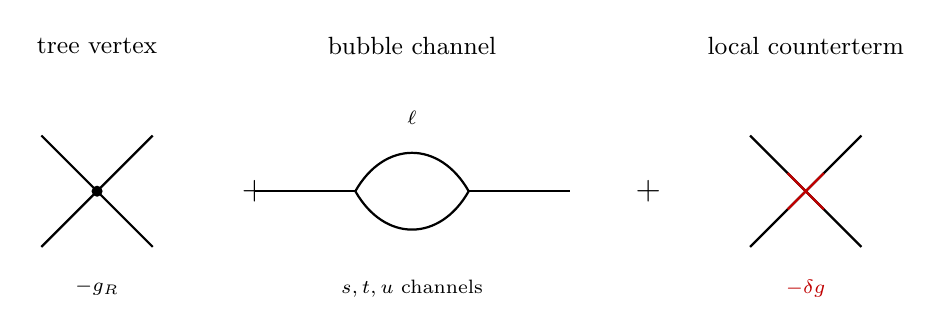
\begin{tikzpicture}[x=1cm,y=1cm,every node/.style={font=\scriptsize}]
    \begin{scope}
      \node[font=\small] at (0,1.85) {tree vertex};
      \foreach \a in {45,135,225,315} {
        \draw[thick] (0,0)--++({1.0*cos(\a)},{1.0*sin(\a)});
      }
      \fill[black] (0,0) circle (2pt);
      \node[below] at (0,-1.0) {\(-g_R\)};
    \end{scope}

    \node[font=\large] at (2.0,0) {\(+\)};

    \begin{scope}[shift={(4.0,0)}]
      \node[font=\small] at (0,1.85) {bubble channel};
      \draw[thick] (-2.0,0)--(-0.72,0);
      \draw[thick] (0.72,0)--(2.0,0);
      \draw[thick] (-0.72,0)..controls (-0.35,0.65) and (0.35,0.65)..(0.72,0);
      \draw[thick] (-0.72,0)..controls (-0.35,-0.65) and (0.35,-0.65)..(0.72,0);
      \node[above] at (0,0.72) {\(\ell\)};
      \node[below] at (0,-1.0) {\(s,t,u\) channels};
    \end{scope}

    \node[font=\large] at (7.0,0) {\(+\)};

    \begin{scope}[shift={(9.0,0)}]
      \node[font=\small] at (0,1.85) {local counterterm};
      \foreach \a in {45,135,225,315} {
        \draw[thick] (0,0)--++({1.0*cos(\a)},{1.0*sin(\a)});
      }
      \draw[red!75!black, thick] (-0.23,-0.23)--(0.23,0.23);
      \draw[red!75!black, thick] (-0.23,0.23)--(0.23,-0.23);
      \node[red!75!black, below] at (0,-1.0) {\(-\delta g\)};
    \end{scope}
  \end{tikzpicture}
  }
  \caption{The one-loop scalar quartic coordinate receives the tree vertex,
  the three bubble channels, and the local quartic counterterm fixed by the
  chosen subtraction condition.}
  \label{fig:volume-ii-phi-four-one-loop-rg}
\end{figure}

With a momentum cutoff \(\Lambda\), the one-loop relation at the symmetric
subtraction point is
\[
\begin{aligned}
  -g(\mu)
  &=
  -g_R-\delta g
  +
  3\frac{g_R^2}{32\pi^2}
  \int_0^1 \dd x\,
  \left[
    \log\frac{\Lambda^2}{m_R^2-sx(1-x)}-1
  \right]_{s=-\frac43\mu^2}
  +
  O(g_R^3).
\end{aligned}
\]
Choose the finite convention
\[
  g_R=g(0).
\]
This condition fixes \(\delta g\).  Subtracting the \(\mu=0\) equation from
the equation at general \(\mu\) removes the cutoff and gives
\[
  g(\mu)
  =
  g_R
  -
  \frac{3g_R^2}{32\pi^2}
  \int_0^1 \dd x\,
  \log
  \frac{m_R^2}
       {m_R^2+\frac43\mu^2x(1-x)}
  +
  O(g_R^3).
\]
This is a finite relation between two renormalized quartic coordinates in the
same theory.  For \(\mu\gg m_R\), the displayed correction contains a large
logarithm.  A comparison built from nearby scale coordinates is then better
adapted to perturbation theory.

\section{Nearby Scales and the Beta Function}

Let \(\mu'\) be close to \(\mu\).  The same one-loop computation may be
expressed as a relation between the two scale coordinates:
\[
  g(\mu')
  =
  g(\mu)
  -
  \frac{3}{32\pi^2}g(\mu)^2
  \int_0^1 \dd x\,
  \log
  \frac{m_R^2+\frac43\mu^2x(1-x)}
       {m_R^2+\frac43\mu'^2x(1-x)}
  +
  O(g(\mu)^3).
\]
The expansion parameter is now \(g(\mu)\), and the logarithm is small for
\(\mu'\) close to \(\mu\).  Setting \(\mu'=\mu+\dd\mu\) gives
\[
  \frac{\dd g(\mu)}{\dd\log\mu}
  =
  \frac{3}{16\pi^2}g(\mu)^2
  \int_0^1\dd x\,
  \frac{\frac43\mu^2x(1-x)}
       {m_R^2+\frac43\mu^2x(1-x)}
  +
  O(g(\mu)^3).
\]
The integral is a threshold factor.  At scales much larger than the mass,
\(\mu\gg m_R\), it tends to \(1\), and
\[
  \frac{\dd g}{\dd\log\mu}
  =
  \frac{3}{16\pi^2}g^2+O(g^3).
\]
In this scheme and convention, the one-loop beta function is therefore
\[
  \beta(g)=\frac{3}{16\pi^2}g^2+O(g^3)
  \qquad
  (\mu\gg m_R).
\]

The one-loop differential equation can be integrated between two scales:
\[
  \frac1{g(\mu)}-\frac1{g(\mu')}
  =
  -\frac{3}{16\pi^2}\log\frac{\mu}{\mu'} .
\]
Equivalently,
\[
  g(\mu)
  =
  \frac{g(\mu')}
       {1-\frac{3}{16\pi^2}g(\mu')\log(\mu/\mu')} .
\]
This expression contains powers of
\(g(\mu')\log(\mu/\mu')\) to all orders.  Its perturbative domain is controlled
by the running coordinate itself: \(g(\widetilde\mu)\) must remain small for
the scales \(\widetilde\mu\) used in the comparison.

\section{The Landau Scale as a Perturbative Coordinate}

The integrated one-loop equation may be written in terms of a scale
\(\mu_0\) defined by
\[
  \mu_0
  =
  \mu'\exp\!\left[
    \frac{16\pi^2}{3g(\mu')}
  \right].
\]
Then
\[
  g(\mu)
  =
  \frac{1}{\frac{3}{16\pi^2}\log(\mu_0/\mu)} .
\]
For \(0<\mu\ll\mu_0\), the denominator is large and the one-loop coordinate is
small.  As \(\mu\) approaches \(\mu_0\), the perturbative coordinate becomes
large and the one-loop approximation ceases to provide a controlled
description.  Within the one-loop equation, the pair
\((\mu',g(\mu'))\) is equivalently represented by the single scale \(\mu_0\).

\begin{figure}[H]
  \centering
  \resizebox{0.70\textwidth}{!}{%
  \begin{tikzpicture}[x=1cm,y=1cm,every node/.style={font=\scriptsize}]
    \draw[-{Latex[length=2mm]}] (-3.0,0)--(3.25,0) node[below] {\(\log\mu\)};
    \draw[-{Latex[length=2mm]}] (-2.65,-0.1)--(-2.65,3.35)
      node[left] {\(g(\mu)\)};
    \draw[blue!70!black, very thick, domain=-2.35:2.35, samples=160]
      plot (\x,{0.55/(2.65-\x)});
    \draw[red!75!black, dashed, thick] (2.65,0)--(2.65,3.05);
    \node[red!75!black, above] at (2.65,3.05) {\(\mu_0\)};
    \node[green!45!black, align=center] at (-1.35,0.72)
      {controlled\\\(g\ll1\)};
    \node[orange!85!black, align=center] at (1.15,1.85)
      {large logarithms\\resummed by RG};
    \node[red!75!black, align=left, anchor=west] at (2.82,1.25)
      {large\\coordinate};
  \end{tikzpicture}
  }
  \caption{The one-loop scalar quartic flow grows with the Euclidean momentum
  scale.  The scale \(\mu_0\) is where the one-loop coordinate diverges; the
  controlled perturbative domain is the region where the running coordinate
  remains small.}
  \label{fig:volume-ii-phi-four-landau-scale}
\end{figure}

\begin{remark}[Status of the Landau scale]
The scale \(\mu_0\) is a statement about the one-loop perturbative coordinate.
It gives a useful parametrization of the weak-coupling region and indicates
where that coordinate loses perturbative control.  A statement about the
existence or nonexistence of a continuum scalar theory at arbitrarily short
distances requires additional nonperturbative input.
\end{remark}

\section{General 1PI Coordinates}

Let a regulated Euclidean action be written as
\[
  S_\Lambda[\phi]
  =
  S_{\rm kin,\Lambda}[\phi]
  +
  \int \dd^Dx\,\sum_I g_I^{\rm bare}(\Lambda)\,\mathcal O_I(x).
\]
For each label \(I\), let \(\mathcal O_I\) be a local operator with mass
dimension \(d_I\), field number \(n_I\), and derivative tensor structure
specified by a polynomial \(P_I\) in external momenta.  The corresponding 1PI
coordinate at scale \(\mu\) is extracted from the \(n_I\)-point vertex by
\[
  g_I(\mu)
  =
  \Pi_I
  \left[
    Z(\mu)^{n_I/2}\,
    \Gamma^{(n_I)}(k_1,\ldots,k_{n_I})
  \right]_{\mathcal S_{I,\mu}} .
\]
The projector \(\Pi_I\) includes the sign and tensor normalization
conventions.  In the scalar quartic example, \(\Pi_I\) is multiplication by
\(-1\) at the symmetric four-point configuration.

The finite comparison of nearby scales gives
\[
  \frac{\dd g_I(\mu)}{\dd\log\mu}
  =
  \beta_I(\{g_J(\mu)\};\mu).
\]
Since \(g_I\) has engineering dimension \(D-d_I\), define the dimensionless
coordinate
\[
  \lambda_I(\mu)
  =
  \mu^{d_I-D}g_I(\mu).
\]
When the coordinate list contains all dimensionless ratios relevant to the
chosen family of theories, the equations may be written as
\[
  \frac{\dd\lambda_I}{\dd\log\mu}
  =
  \beta_I(\{\lambda_J\}).
\]
This autonomous form is a coordinate statement: the beta functions depend on
the selected operator basis, subtraction configurations, field normalization,
and finite part conventions.

The practical value of the 1PI RG is logarithmic organization.  A fixed-order
comparison between two widely separated scales can contain powers of
\(\log(\mu/\mu')\).  The differential equation breaks that comparison into
small steps and then integrates the result, thereby summing the logarithmic
terms determined by the computed beta function.

\section{Callan--Symanzik Equation}

The beta function is a vector field on the renormalized coordinate space.  Its
action on correlation functions is the Callan--Symanzik equation.  Let
\(\phi_R=Z_\phi(\mu)^{-1/2}\phi_0\) be a renormalized scalar field, and let
\[
  G_R^{(n)}(x_1,\ldots,x_n;\lambda(\mu),\mu)
  =
  \langle
    \phi_R(x_1)\cdots\phi_R(x_n)
  \rangle
\]
be a renormalized connected correlation function in a one-coupling family.
The bare correlation function is independent of the auxiliary scale \(\mu\).
Define
\[
  \gamma_\phi(\lambda)
  =
  \frac12\frac{\dd\log Z_\phi}{\dd\log\mu}.
\]
Then
\begin{equation}
  \left(
    \mu\frac{\partial}{\partial\mu}
    +
    \beta(\lambda)\frac{\partial}{\partial\lambda}
    +
    n\gamma_\phi(\lambda)
  \right)
  G_R^{(n)}
  =
  0.
  \label{eq:callan-symanzik-connected}
\end{equation}
The derivative \(\mu\partial_\mu\) is taken at fixed coordinates \(x_i\) and
fixed value of the renormalized coordinate \(\lambda\); the second term moves
the theory point along the RG vector field.

For several couplings the equation is
\[
  \left(
    \mu\frac{\partial}{\partial\mu}
    +
    \sum_I\beta_I(\lambda)\frac{\partial}{\partial\lambda_I}
    +
    n\gamma_\phi(\lambda)
  \right)G_R^{(n)}=0.
\]
For a collection of operators \(\mathcal O_A\), the last term is replaced by
the anomalous-dimension matrix acting on the operator labels.  Thus scaling
laws at a fixed point are obtained by diagonalizing the linear action of the
RG on local operators, while running away from a fixed point is governed by
the full vector field \(\beta_I\partial_{\lambda_I}\).

\section{Logarithmic Consistency}

The existence of finite beta functions imposes relations among logarithms in
cutoff perturbation theory.  Let
\[
  L=\log\frac{\Lambda}{\mu},
\]
and suppose a one-coupling coordinate has the bare expansion
\[
  g(\mu)
  =
  g_0-b_1g_0^2L-b_2g_0^3L-c_1g_0^3L^2+O(g_0^4).
\]
Since \(\dd L/\dd\log\mu=-1\),
\[
  \frac{\dd g(\mu)}{\dd\log\mu}
  =
  b_1g_0^2+b_2g_0^3+2c_1g_0^3L+O(g_0^4).
\]
Inverting the first displayed relation to the order needed gives
\[
  g_0=g(\mu)+b_1g(\mu)^2L+O(g(\mu)^3).
\]
Therefore
\[
  \frac{\dd g(\mu)}{\dd\log\mu}
  =
  b_1g(\mu)^2+b_2g(\mu)^3
  +
  2\bigl(c_1+b_1^2\bigr)g(\mu)^3L
  +
  O(g(\mu)^4).
\]
A beta function expressed in terms of the renormalized coordinate must be
finite as the cutoff is removed.  Hence the explicit \(L\)-term at this order
vanishes:
\[
  c_1=-b_1^2.
\]

\begin{figure}[H]
  \centering
  \resizebox{0.86\textwidth}{!}{%
  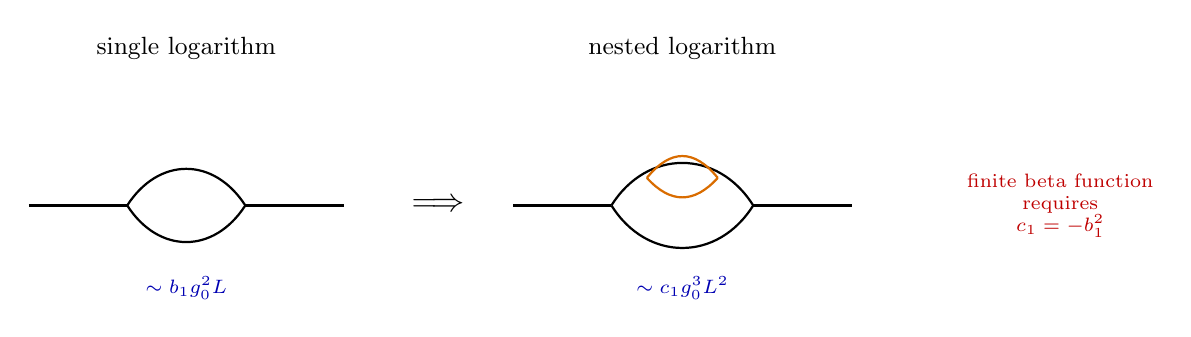
\begin{tikzpicture}[x=1cm,y=1cm,every node/.style={font=\scriptsize}]
    \begin{scope}
      \node[font=\small] at (0,2.0) {single logarithm};
      \draw[thick] (-2.0,0)--(-0.75,0);
      \draw[thick] (0.75,0)--(2.0,0);
      \draw[thick] (-0.75,0)..controls (-0.35,0.62) and (0.35,0.62)..(0.75,0);
      \draw[thick] (-0.75,0)..controls (-0.35,-0.62) and (0.35,-0.62)..(0.75,0);
      \node[blue!70!black] at (0,-1.05) {\(\sim b_1 g_0^2 L\)};
    \end{scope}

    \node[font=\large] at (3.2,0) {\(\Longrightarrow\)};

    \begin{scope}[shift={(6.3,0)}]
      \node[font=\small] at (0,2.0) {nested logarithm};
      \draw[thick] (-2.15,0)--(-0.9,0);
      \draw[thick] (0.9,0)--(2.15,0);
      \draw[thick] (-0.9,0)..controls (-0.45,0.72) and (0.45,0.72)..(0.9,0);
      \draw[thick] (-0.9,0)..controls (-0.45,-0.72) and (0.45,-0.72)..(0.9,0);
      \draw[orange!85!black, thick] (-0.45,0.35)..controls (-0.15,0.72) and
        (0.15,0.72)..(0.45,0.35);
      \draw[orange!85!black, thick] (-0.45,0.35)..controls (-0.15,0.02) and
        (0.15,0.02)..(0.45,0.35);
      \node[blue!70!black] at (0,-1.05) {\(\sim c_1g_0^3L^2\)};
    \end{scope}

    \node[align=center, red!75!black] at (11.1,0)
      {finite beta function\\requires\\\(c_1=-b_1^2\)};
  \end{tikzpicture}
  }
  \caption{The double logarithm associated with nested one-loop subgraphs is
  constrained by the one-loop beta function.  Its coefficient is fixed by the
  requirement that the beta function, expressed in the renormalized coordinate,
  have a finite cutoff-removal limit.}
  \label{fig:volume-ii-double-log-consistency}
\end{figure}

This calculation is the scale-differential form of the locality statements
from the previous chapters.  The logarithm associated with a subgraph can be
reused inside a larger graph, and the coefficient of the resulting double
logarithm is determined by the lower-order beta function rather than by an
independent datum.

\section{Scheme Changes}

A renormalization scheme is a coordinate system on the renormalized family of
theories.  Let \(\lambda\) and \(\widetilde\lambda\) be two coordinates related
by a finite redefinition
\[
  \widetilde\lambda=f(\lambda)
  =
  \lambda+\alpha\lambda^2+O(\lambda^3),
\]
where \(f'(0)=1\).  If
\[
  \frac{\dd\lambda}{\dd\log\mu}=\beta(\lambda),
  \qquad
  \frac{\dd\widetilde\lambda}{\dd\log\mu}
  =
  \widetilde\beta(\widetilde\lambda),
\]
then the chain rule gives
\[
  \widetilde\beta(f(\lambda))=f'(\lambda)\beta(\lambda),
  \qquad
  \beta(\lambda)=\frac{\widetilde\beta(f(\lambda))}{f'(\lambda)}.
\]
Expanding to first order in the finite redefinition parameter,
\[
  \beta(\lambda)
  =
  \widetilde\beta(\lambda)
  +
  \alpha\lambda
  \left(
    \lambda\frac{\partial}{\partial\lambda}-2
  \right)
  \widetilde\beta(\lambda)
  +
  O(\alpha^2).
\]
For one classically marginal coordinate,
\[
  \beta(\lambda)=b_1\lambda^2+b_2\lambda^3+b_3\lambda^4+\cdots,
  \qquad
  \widetilde\beta(\lambda)
  =
  \widetilde b_1\lambda^2+\widetilde b_2\lambda^3
  +\widetilde b_3\lambda^4+\cdots .
\]
The relation above implies
\[
  b_1=\widetilde b_1,
  \qquad
  b_2=\widetilde b_2,
  \qquad
  \widetilde b_3=b_3-\alpha b_2
\]
for the displayed redefinition.  Thus the first two coefficients are invariant
for a single marginal coupling under such finite reparametrizations, while
later coefficients are coordinate dependent.

\section{Invariant Data at Fixed Points}

The preceding one-coordinate computation is a special case of the tensorial
transformation law for a vector field.  Let \(\mathcal T\) be a finite
dimensional coordinate patch in the renormalized theory family, with local
coordinates \(\lambda^I\).  The beta function is the vector field
\[
  \beta=\beta^I(\lambda)\frac{\partial}{\partial\lambda^I}.
\]
A finite scheme change is a local diffeomorphism
\[
  \widetilde\lambda^A=f^A(\lambda),
  \qquad
  J^A{}_I(\lambda)=\frac{\partial f^A}{\partial\lambda^I}.
\]
The components of the same vector field in the new coordinates are
\[
  \widetilde\beta^A(\widetilde\lambda)
  =
  J^A{}_I(\lambda)\,\beta^I(\lambda),
  \qquad
  \widetilde\lambda=f(\lambda).
\]
Thus a beta function is not a coordinate-independent list of functions; the
coordinate-independent object is the flow it defines on \(\mathcal T\).

A fixed point is a zero of this vector field:
\[
  \beta^I(\lambda_\ast)=0 .
\]
This statement is invariant under changes of coordinates.  Let
\[
  M^I{}_J
  =
  \left.
  \frac{\partial\beta^I}{\partial\lambda^J}
  \right|_{\lambda_\ast}
\]
be the linearization of the RG vector field at the fixed point.  Since the
extra term obtained by differentiating \(J^A{}_I(\lambda)\beta^I(\lambda)\)
is proportional to \(\beta(\lambda_\ast)\), it vanishes at the fixed point.
Therefore
\[
  \widetilde M^A{}_B
  =
  J^A{}_I(\lambda_\ast)\,
  M^I{}_J\,
  (J^{-1})^J{}_B(\lambda_\ast).
\]
The linearized matrices in two schemes are similar.  Their eigenvalues are
therefore invariant, although their eigenvectors are represented by different
coordinate components.  These eigenvalues are the critical exponents of the
linearized flow in the chosen normalization of RG time.

If \(M\) has zero eigenvalues, the linearized analysis identifies tangent
directions that require higher-order study.  A zero eigenvalue is the
condition for linearized marginality; exact marginality is the stronger
statement that the RG vector field vanishes along an actual submanifold of
theory space.  In local QFT this statement must also be made after quotienting
redundant directions generated by field redefinitions and after imposing the
symmetries used to define the coordinate patch.

\begin{figure}[H]
  \centering
  \resizebox{0.76\textwidth}{!}{%
  \begin{tikzpicture}[x=1cm,y=1cm,every node/.style={font=\scriptsize}]
    \node[draw=black, rounded corners, align=center, inner sep=7pt]
      (A) at (-2.8,0) {coordinate \(\lambda\)\\\(\beta(\lambda)\)};
    \node[draw=black, rounded corners, align=center, inner sep=7pt]
      (B) at (2.8,0) {coordinate \(\widetilde\lambda\)\\
      \(\widetilde\beta(\widetilde\lambda)\)};
    \draw[-{Latex[length=2mm]}, thick] (A) -- node[above]
      {\(\widetilde\lambda=f(\lambda)\)} (B);
    \draw[-{Latex[length=2mm]}, thick] (B) to[bend left=18]
      node[below] {\(\beta=\widetilde\beta\circ f/f'\)} (A);
    \node[align=center, blue!70!black] at (0,-1.55)
      {same renormalized family\\different finite coordinates};
  \end{tikzpicture}
  }
  \caption{A finite scheme change is a change of coordinates on the
  renormalized theory family.  The beta function transforms as a vector field
  under this change of coordinate.}
  \label{fig:volume-ii-scheme-change}
\end{figure}

The next chapter applies the same scale-dependent logic to local operator
insertions.  Infinitesimal deformations of the action define renormalized
operators, and their scale dependence is governed by the linearization of the
beta-function vector field.
